% \chapter{补充更多细节}

% \section{补充图}

% \subsection{补充图}

% 这是附录内容,应该用宋体小四号字体。
% \begin{figure}[htbp]
%         \centering
%         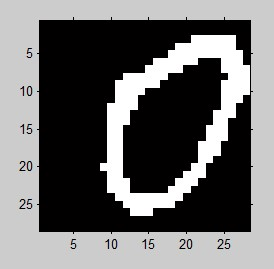
\includegraphics[height=6.54cm]{image/chap04/1.jpg}
%         \caption{实验训练集}
% \end{figure}
% \begin{figure}
%         \centering
%         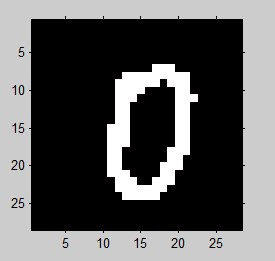
\includegraphics[height=6.54cm]{image/chap04/2.jpg}
%         \caption{实验测试集}
% \end{figure}

\chapter{其他图类型}

\paragraph*{小世界图(Small World)}
\begin{figure}[tb]
    \centering
    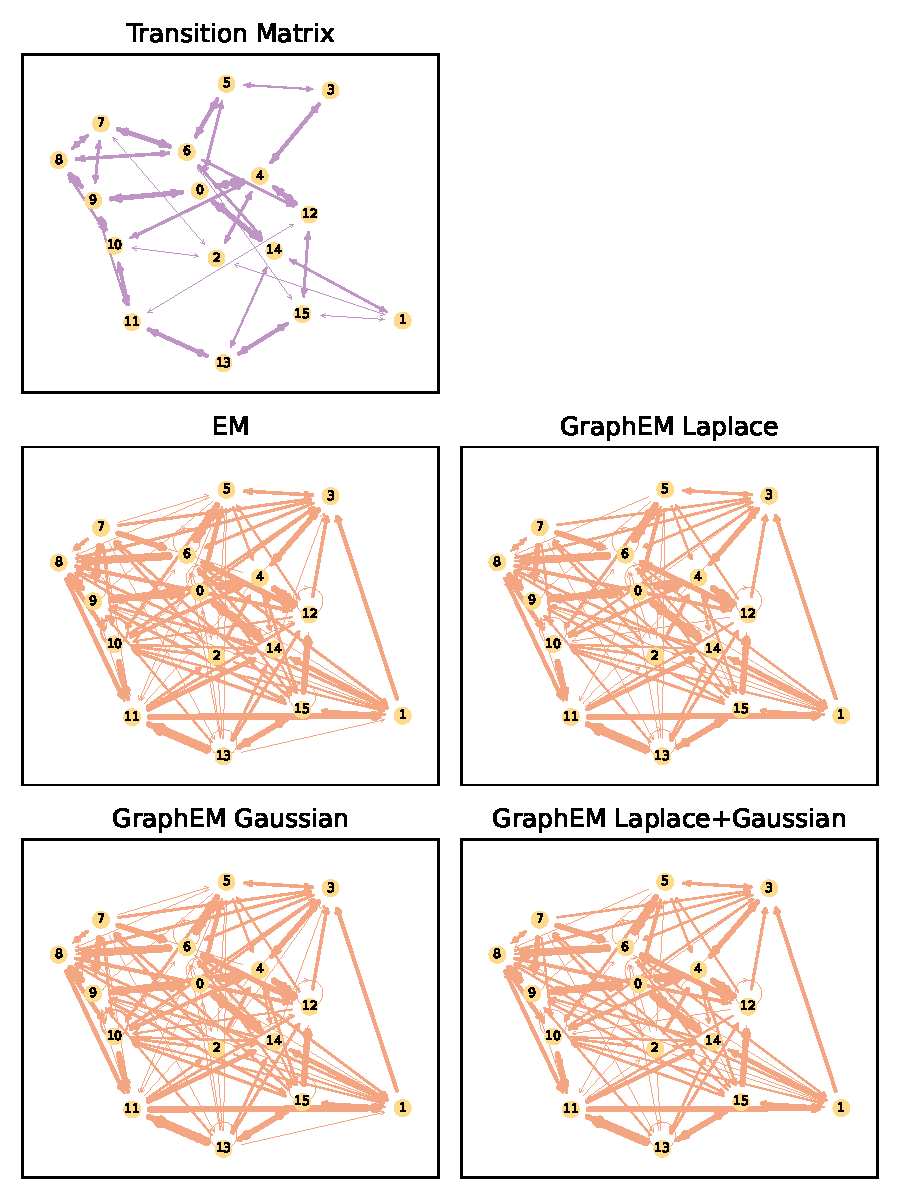
\includegraphics[width=0.75\linewidth]{fig/small world/graphs_for_true_and_EM.pdf}
    \caption{小世界图的真实转移矩阵与估计矩阵对比图。}
    \label{fig: small world graph comparison}
\end{figure}

图~\ref{fig: small world graph comparison} 对比了小世界图的真实转移矩阵与估计矩阵。结果表明,GraphEM 的 Laplace+Gaussian 方法能够有效捕捉小世界网络所特有的局部聚类与远程连接特性,其表现优于其他正则化策略。

\paragraph*{无标度图(Scale Free)}
\begin{figure}[tb]
    \centering
    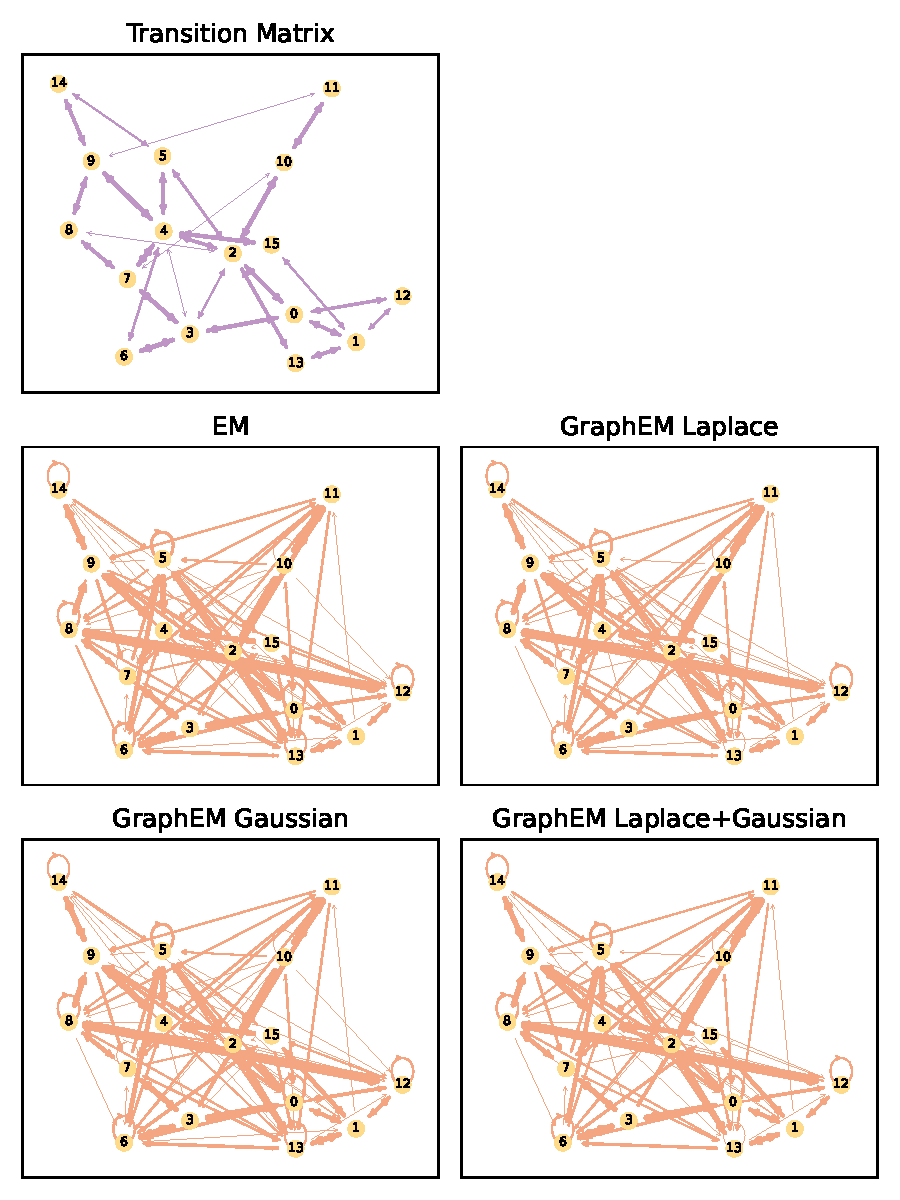
\includegraphics[width=0.75\linewidth]{fig/scale free/graphs_for_true_and_EM.pdf}
    \caption{无标度图的真实转移矩阵与估计矩阵对比图。}
    \label{fig: scale free graph comparison}
\end{figure}

图~\ref{fig: scale free graph comparison} 展示了无标度图的真实与估计转移矩阵。GraphEM Laplace+Gaussian 方法在识别枢纽节点和保持幂律度分布方面表现出色,显示出其在处理无标度结构时的鲁棒性。

\paragraph*{二部图(Bipartite)}
\begin{figure}[tb]
    \centering
    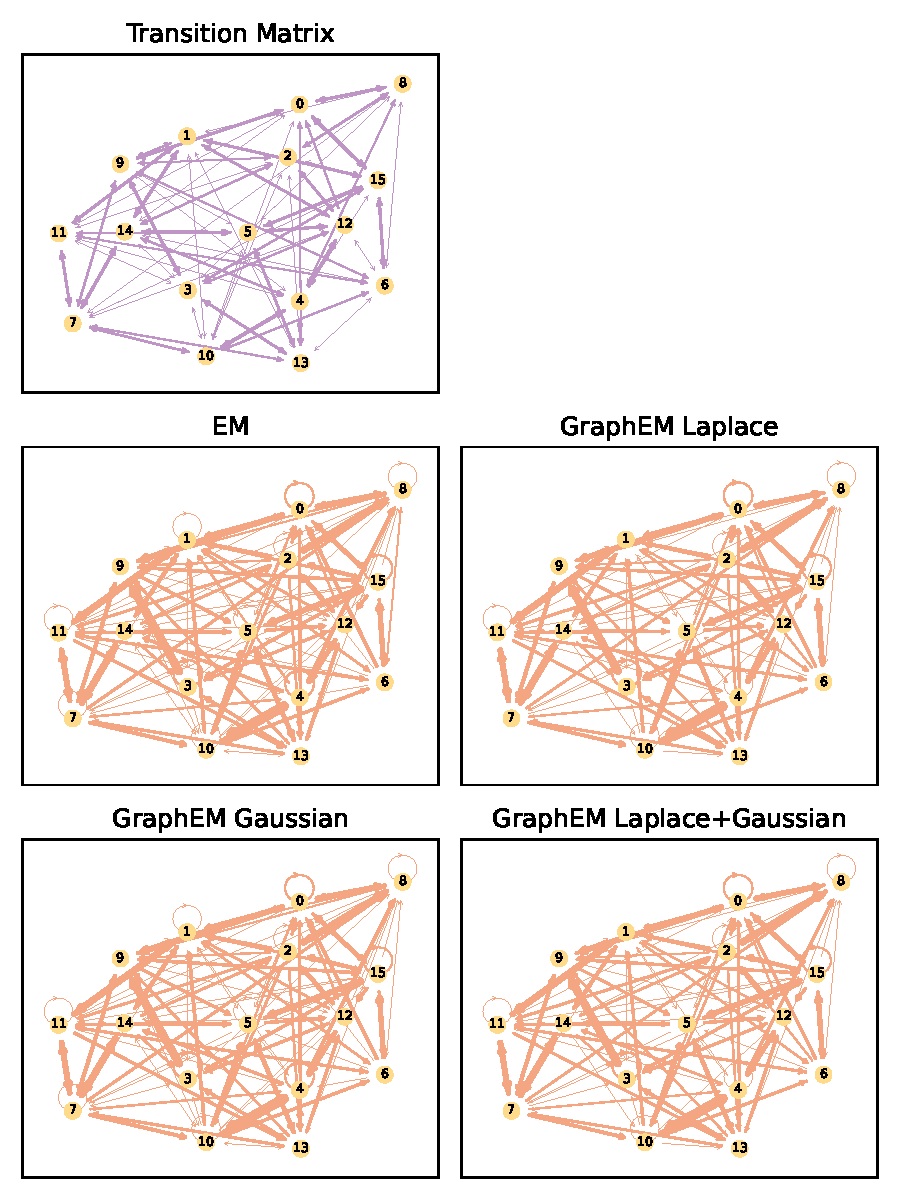
\includegraphics[width=0.75\linewidth]{fig/bipartite/graphs_for_true_and_EM.pdf}
    \caption{二部图的真实转移矩阵与估计矩阵对比图。}
    \label{fig: bipartite graph comparison}
\end{figure}

图~\ref{fig: bipartite graph comparison} 展示了二部图的真实与估计转移矩阵。GraphEM Laplace+Gaussian 方法能够准确捕捉二部结构,展现了其建模不同节点集合之间关系的能力。

\paragraph*{环图(Cycle)}
\begin{figure}[tb]
    \centering
    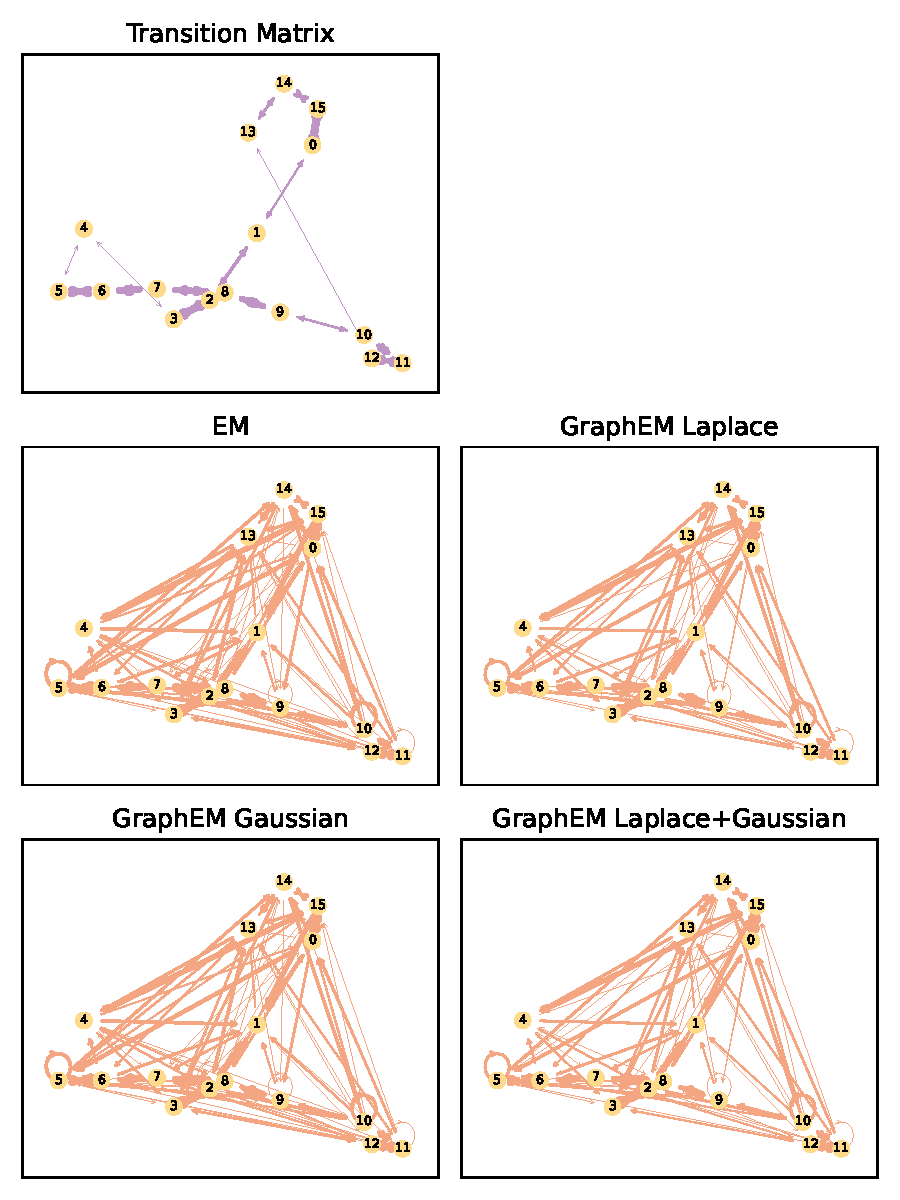
\includegraphics[width=0.75\linewidth]{fig/cycle/graphs_for_true_and_EM.pdf}
    \caption{环图的真实转移矩阵与估计矩阵对比图。}
    \label{fig: cycle graph comparison}
\end{figure}

图~\ref{fig: cycle graph comparison} 对比了环图的真实与估计转移矩阵。GraphEM Laplace+Gaussian 方法有效保留了环状结构,展现了其建模周期性关系的能力。

\paragraph*{星型图(Star)}
\begin{figure}[tb]
    \centering
    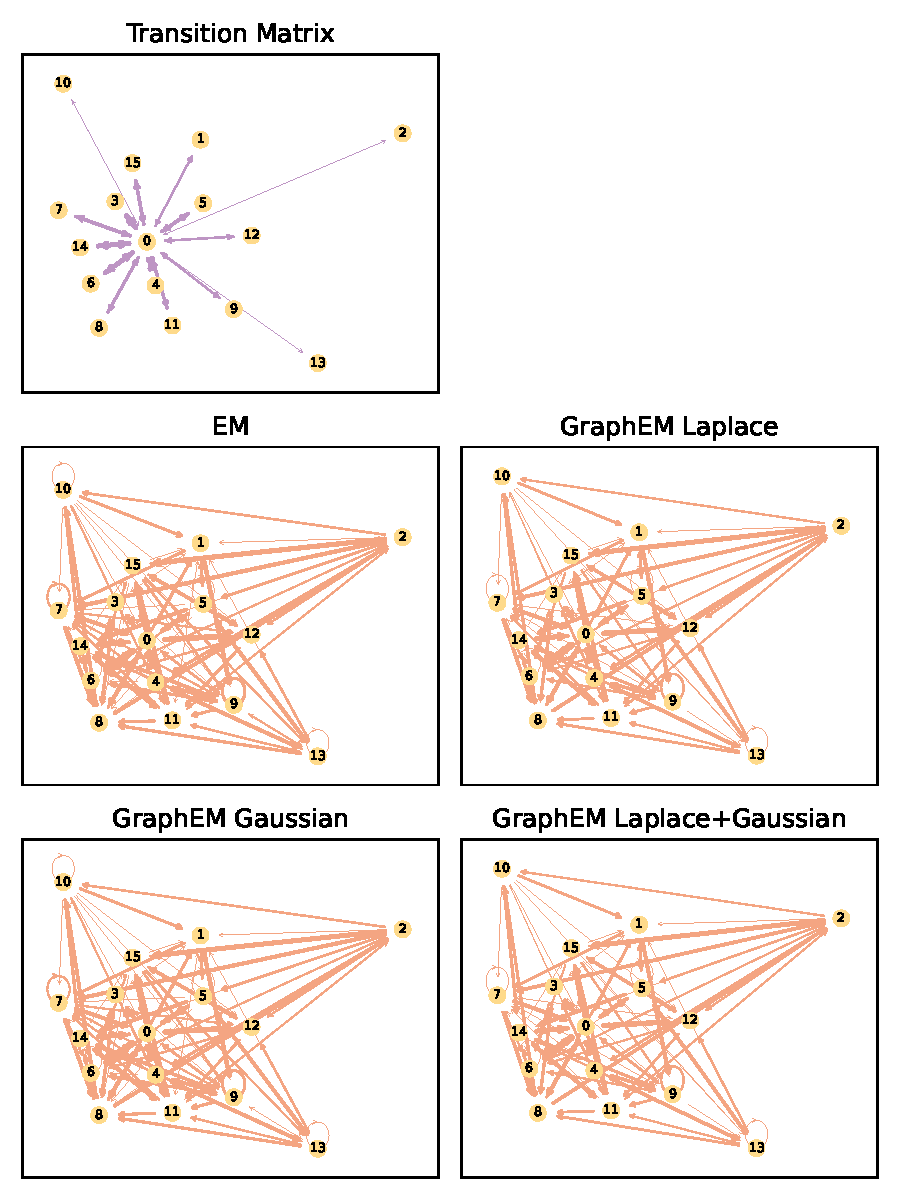
\includegraphics[width=0.75\linewidth]{fig/star/graphs_for_true_and_EM.pdf}
    \caption{星型图的真实转移矩阵与估计矩阵对比图。}
    \label{fig: star graph comparison}
\end{figure}

图~\ref{fig: star graph comparison} 展示了星型图的真实与估计转移矩阵。GraphEM Laplace+Gaussian 方法能够准确识别中心节点及其与边缘节点的连接,展现出其在建模星状网络中的有效性。

\endinput
